\section{�C�mo empiezo?}

\subsection{Modo de funcionamiento}

\begin{frame}{El funcionamiento de \LaTeX{}}
\begin{enumerate}
\item <1-> \alert<1>{Escribir el contenido \textbf<1>{estructurado} mediante el \textbf<1>{lenguaje} marcado}
\item <2-> \alert<2>{Se \textbf<2>{compila}, y \LaTeX{} se encarga de \textbf<2>{dar formato} al texto}
\item <3-> \alert<3>{\textbf<3>{Visualizaci�n} por pantalla del fichero resultante}
\end{enumerate}
\only<4->{
\begin{figure}[hbtp]
\centering
\begin{tikzpicture}
\alt<4->{\node[opacity=1]{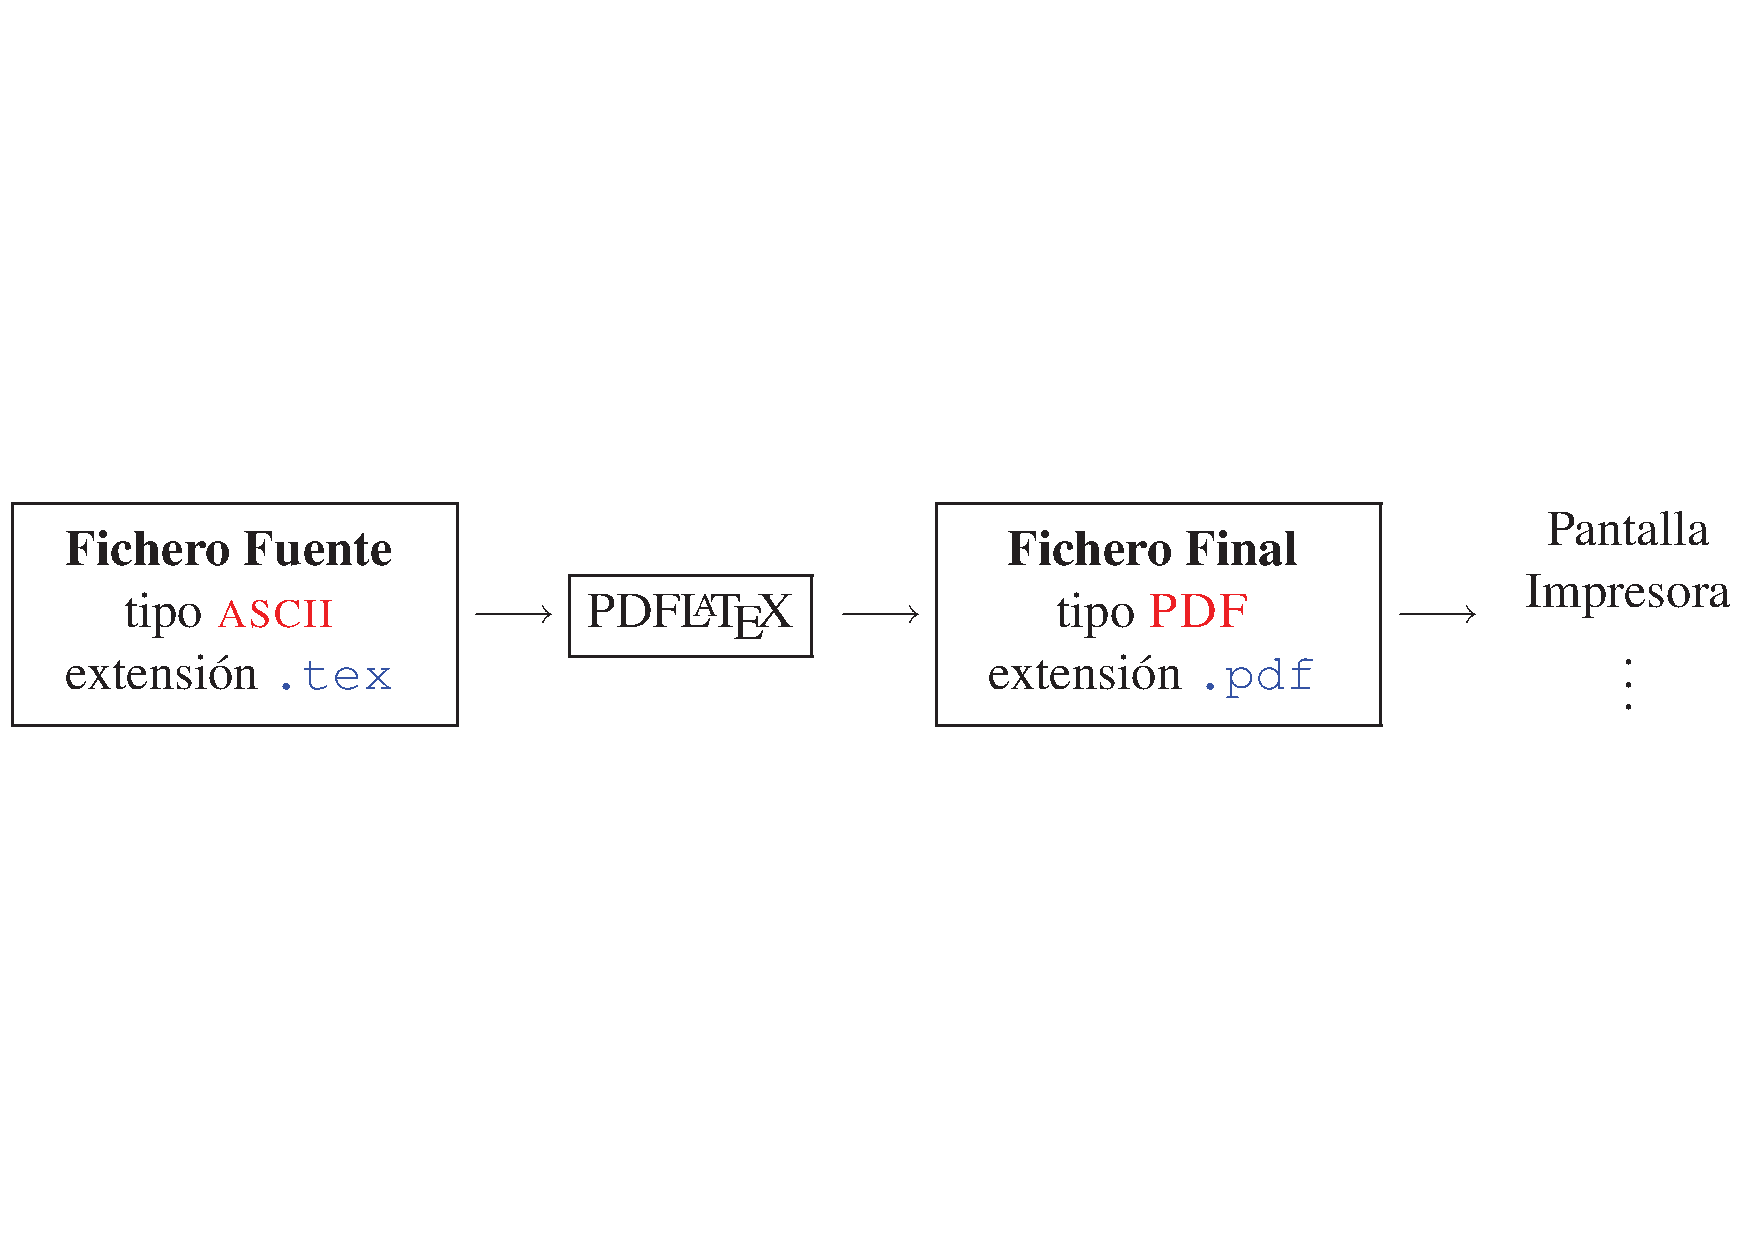
\includegraphics[width=\textwidth]{Figuras/funcionamiento}};}
{\node[opacity=0.01]{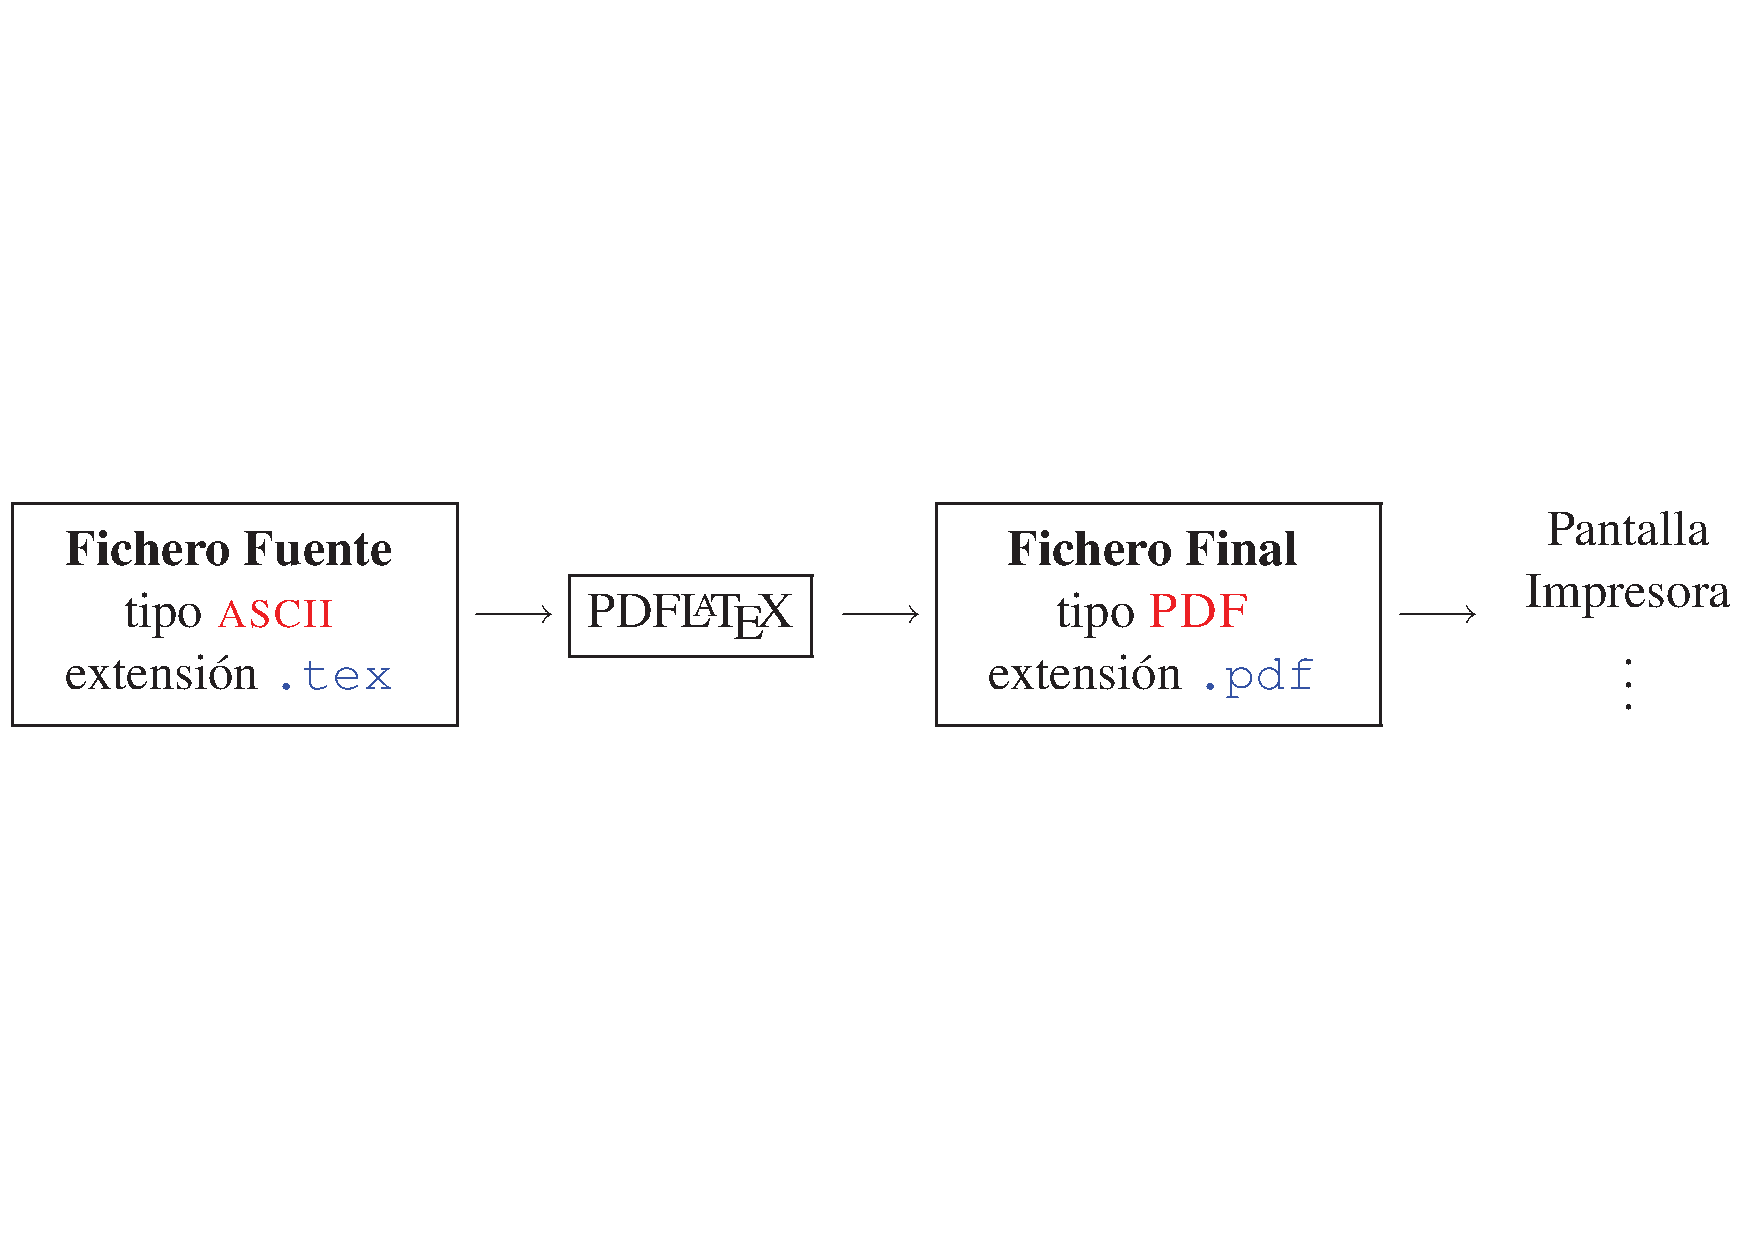
\includegraphics[width=\textwidth]{Figuras/funcionamiento}};}
\end{tikzpicture}
\vspace{-0.75cm}
\visible<4->{\caption{Modo de funcionamiento de \LaTeX{} (PDF\LaTeX{})}}
\label{fig:CurvaAprendizaje}
\end{figure}}
\end{frame}

\subsection{Los requerimientos}
\begin{frame}{Los  requerimientos}
Necesitaremos tener instalado en nuestro ordenador:
\begin{itemize}
\item<2-> \alert<2>{Acrobar Reader}
\item<3-> \alert<3>{Una distribuci�n de \TeX{} y \LaTeX{}:}
\visible<4->{\begin{itemize}
\item Para Windows: MiK\TeX
\item Para Linux/Unix: te\TeX
\item Para MacOSX: \TeX Shop
\end{itemize} }
\end{itemize}
\visible<5->{Cualquiera de estas distribuciones posee:}
\visible<6->{
\begin{itemize}
\item<6->  \alert<6>{Ventana de editor}
\item<7-> \alert<7>{Ventana de compilaci�n (para visualizar pasos, errores y precauciones (\textbf<8>{\em warnings}))}
\item<8-> \alert<8>{Ventana de visualizaci�n del fichero generado}
\end{itemize}}
\end{frame}